\documentclass{article}
\usepackage{graphicx}
\usepackage{caption}
\usepackage{subcaption}
\usepackage{wrapfig}

\begin{document}
	
	Each image is pre-processed to reduce the resolution, condensing a cell in one pixel, while maintaining its basic shape to avoid any collision. (Fig 1) \\*
	
	\begin{tabbing}
		\textbf{for each} cell in image \\*
		\kern 1pc \textbf{for each} pixel in cell\\*
		\kern 2pc \textbf{if} at least one pixel is true \textbf{then} \\*
		\kern 3pc corresponding grid cell is true \\*
	\end{tabbing}
	
	\begin{figure}[h]
		\centering
		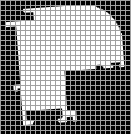
\includegraphics[width=0.3\linewidth]{gridoverlay}
		\caption{Grid overlay}
	\end{figure}
	
	\begin{figure}[h]
		\centering
		\begin{subfigure}{0.5\textwidth}
			\centering
			
\includegraphics[width=0.6\linewidth]{img}
			\caption{Original image}
			\label{fig:img}
		\end{subfigure}%
		\begin{subfigure}{0.5\textwidth}
			\centering
			
\includegraphics[width=0.6\linewidth]{grid}
			\caption{Image grid}
			\label{fig:grid}
		\end{subfigure}
		\caption{A mask before and after being processed}
		\label{fig:test}
	\end{figure}

	Due to the reduced complexity, every check on profile collision is made on grids. \\*
	
	To achieve the greatest possible profile density, each one must be placed on the highest-value free position. \\*
	
	For instance, if the real-world case scenario requires profiles to be stacked on the lower edge, the highest-value point would be the bottom-left corner, decreasing while traversing the image horizontally first, then vertically. (Fig 3) \\*
	
	\begin{figure}[h]
		\centering
		
\includegraphics[width=0.3\linewidth]{value}
		\caption{Value of positions}
		\label{fig:value}
	\end{figure}

	\begin{tabbing}
		\textbf{for each} grid to place \\*
		\kern 1pc \textbf{if} grid collides with existing grid on Result grid \textbf{then} \\*
		\kern 2pc move to next highest-value point \\*
		\kern 1pc \textbf{else} \\*
		\kern 2pc place profile on the Result image/grid at the corresponding coordinates
	\end{tabbing}

	\begin{figure}[h]
		\centering
		\begin{subfigure}{0.5\textwidth}
			\centering
			
\includegraphics[width=0.6\linewidth]{result_grid}
			\caption{Result grid}
			\label{fig:resimg}
		\end{subfigure}%
		\begin{subfigure}{0.5\textwidth}
			\centering
			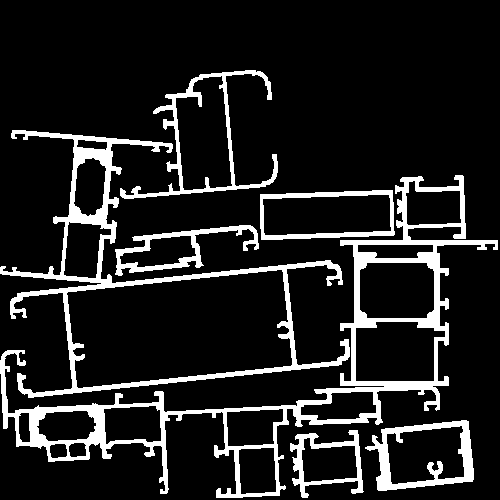
\includegraphics[width=0.6\linewidth]{result_img}
			\caption{Result image}
			\label{fig:resgrid}
		\end{subfigure}
		\caption{Output}
		\label{fig:res}
	\end{figure}
	
\end{document}